\documentclass[12pt, preprint]{aastex}
\usepackage{graphicx}
\usepackage[vmargin=1in,hmargin=1in]{geometry}
\usepackage{natbib}
\usepackage{epsfig}
\setlength{\parindent}{0in}
\newcommand{\ha}{$H\alpha$}
\newcommand{\rtwo}{$R_{200}$}
\newcommand{\size}{$ R_e(24)/R_e(r)$}
\newcommand{\sizeb}{$ R_e(22)/R_e(r)$}
% \newcommand{\dr}{$\Delta R/R_{200}$}
\newcommand{\lcs}{$Local \ Cluster \ Survey $}
\newcommand{\rad}{$R_e$}
\newcommand{\sers}{{\it S\'{e}rsic}}
%\newcommand{\micron}{{$\mu m$}}
%\newcommand{\arcsec}{$"$}

\pagestyle{myheadings}
\markright{Probing Gas in Virgo Filament Galaxies \hfill Rose A. Finn~~}


\begin{document}


%\tableofcontents
%\newpage
\section{Overview}
\vspace*{-.4cm}
We propose to combine multi-wavelength data to probe the gas and dust
in galaxies in two nearby filaments to constrain the physical mechanisms that cause galaxies to evolve from 
blue, actively star-forming galaxies to red, passive galaxies. We will focus on where 
and how passage into a filamentary structure affects a galaxy's gas
supply.  Specifically, we will measure the spatial extent 
of the dust and star-forming disks relative to the stellar disk for $\sim$200
galaxies that reside in the large-scale filaments surrounding the
Virgo cluster.  We will combine this information with measurements of
molecular gas and atomic hydrogen to create a complete census of the
interstellar medium for a large sample of galaxies in this dynamic
environment.  

Virgo is one of the best studied clusters, period.  
We will our gas and dust properties of
filament galaxies with existing measurements of Virgo cluster galaxies
and isolated field galaxies.  
We will compare these results to simulations of cluster growth and
semi-analytic models of gas consumption to help identify the physical mechanisms 
that deplete galactic gas in dense environments, a key aspect required to understand galaxy evolution. 

Most previous studies that look at the influence of environment on
galaxy gas and star formation properties classify environment in terms
of either cluster-centric radius or local density.  However, the
distribution of galaxies is not smooth, even near clusters.  In this
proposal, we move beyond  to look as galaxies along two filaments that
are feeding a group and cluster.


\vspace*{-1cm}
\section{Scientific Motivation}
\vspace*{-.4cm}

%\underline{The Role of Environment in Suppressing Star Formation.}  
A wealth of previous work has established that the fraction of
quiescent (non star-forming) galaxies increases with
stellar mass and environmental density \citep[e.g.][]{dale01,kauffmann04,peng10}.
However, the physical processes that deplete a galaxy's gas content and
thus star formation remain unclear.  
In this proposal, we are focusing on where and how environment affects galaxies.  
While interactions with the intracluster medium clearly strip gas
from some infalling cluster galaxies \citep[e.g.][]{chung07}, there
is ample evidence that galaxy SFRs are suppressed at distances up
to $\sim$5 virial radii from cluster centers \citep{lewis02,bahe13}.  
This suggests that galaxies are being processed by dense environments before they
fall into clusters \citep[e.g.][]{poggianti99,cortese06}.  



% \underline{Probing Star Formation and Molecular Gas.} 
% {\em We propose \ha \ imaging to map the
%   spatial distribution of the hot gas and derive integrated
%   star-formation rates for 20 galaxies in the filament extending to
%   the NE of Virgo (Figure 1).}  We have approved
%   CO(2-1) and (1-0) observations with the IRAM 30-meter telescope to
%   characterize the molecular gas content of these galaxies.   The
% combination of \ha \ and CO observations will allow us to calculate
% gas consumption timescales, characterize multiple phases of the
% galactic gas, and look for signatures of environmentally-driven depletion.



%\underline{Signatures of Quenching Mechanisms.}  
Despite clear evidence for intrinsic and environmental
quenching of star formation, the physical processes underlying these
correlations are not well known. 
Intrinsic processes may quench star formation through
ejection or heating of the gas without impacting the distribution of
existing stars \citep[e.g.][]{springel05,
  croton06, dekel06}.  External or environmentally-driven processes 
such as tidal interactions and
mergers can
affect the distribution of both gas and stars \citep{springel05,
  croton06, dekel06}, whereas pressure-driven interactions are expected to
act primarily on the gas.  For example, starvation, which results from
a galaxy being cutoff from its supply of cold gas \citep{larson80}, is
expected to result in
truncated gas disks while the spatial distribution of the
remaining disk gas is circularly symmetric and the stellar disk is unaffected \citep[e.g.][]{kawata08}. 
The interaction of galactic disk gas with the intracluster medium via
ram-pressure stripping can remove the gas and produce asymmetries in
the remaining disk gas \citep[e.g.][]{quilis00,crowl05}.  
%that disk gas is compressed in the direction of motion  and cupped in
%morphology \citep[e.g.][]{quilis00,crowl05}.  
{The environmental effects thus
have different signatures on the relative abundances and spatial
distribution of the warm ionized gas and molecular gas.  By
observing both 
phases, we can distinguish between these processes.}
 

%\noindent  \underline{Galaxies in the Cosmic Web.}  
Large galaxy redshift surveys have revealed that galaxies are distributed in a complex network
of matter with a large dynamic range of local density, called the
cosmic web or filamentary structures \citep{kitaura09, darvish14}.  These structures are seen in striking clarity around the
Virgo cluster as shown in the top panel of Figure \ref{fig1}.  Our goal is to understand how 
galaxies are altered as they move through the cosmic web and enter the
densest regions.  We are therefore in the midst of a
multi-wavelength study of galaxies at a variety of positions in the
cosmic web surrounding the Virgo cluster, one of the best studied
regions of high density in the Universe.  

background of filaments - galaxies fall into clusters along the
filaments.

galaxies change colors in dense environments.

story - as large scale structure forms,
galaxies in dense environments are different than field environment.
growth of structure must affect galaxy properties.  where is this happening.
simulation picture - red and blue picture - what is relationship 

%\newpage
 \begin{figure}[h]
   \centering
   %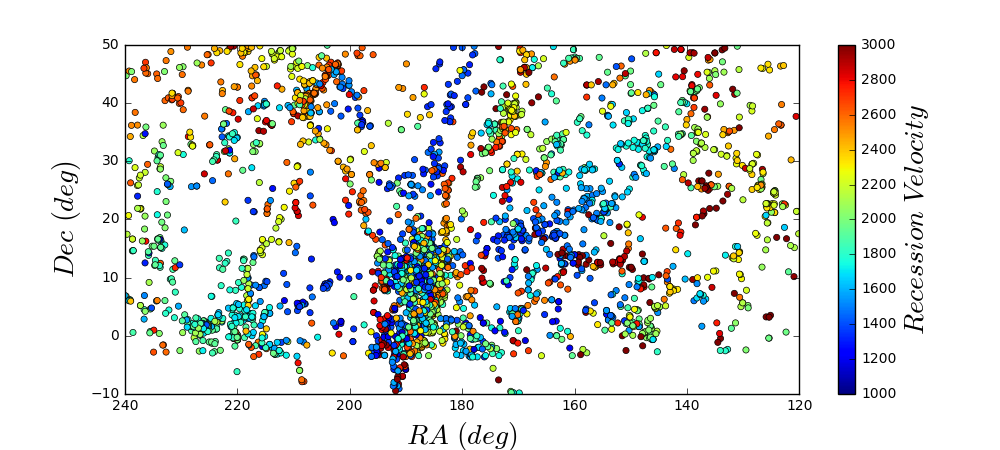
\includegraphics[width=.7\textwidth]{Virgo_positions_NSF.png}
   %\includegraphics[width=0.48\textwidth]{Virgo_filament_Halpha_obs.eps}
 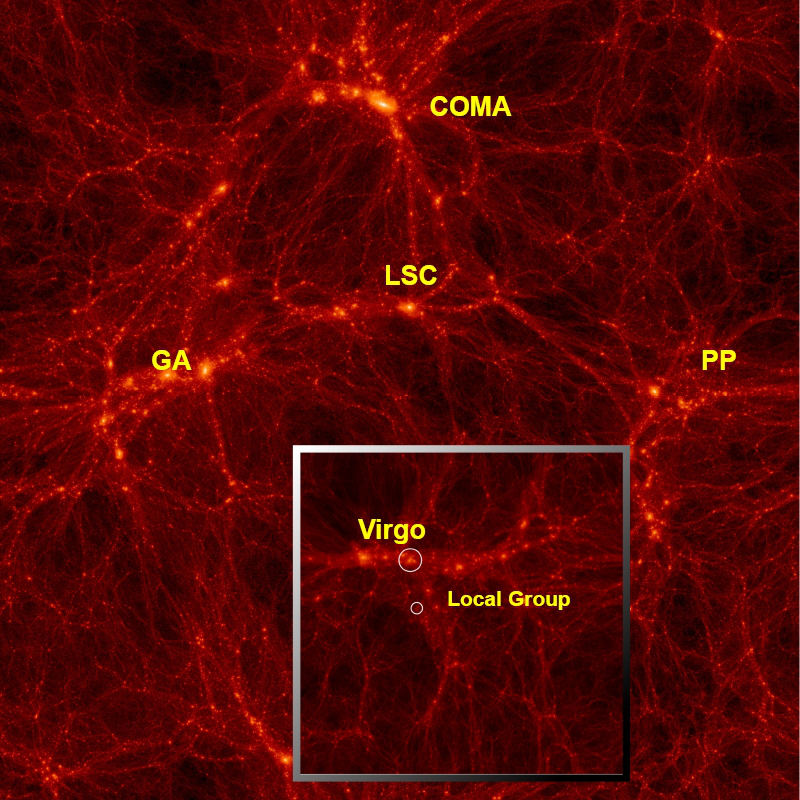
\includegraphics[width=.48\textwidth]{CLUES-DM.png}
 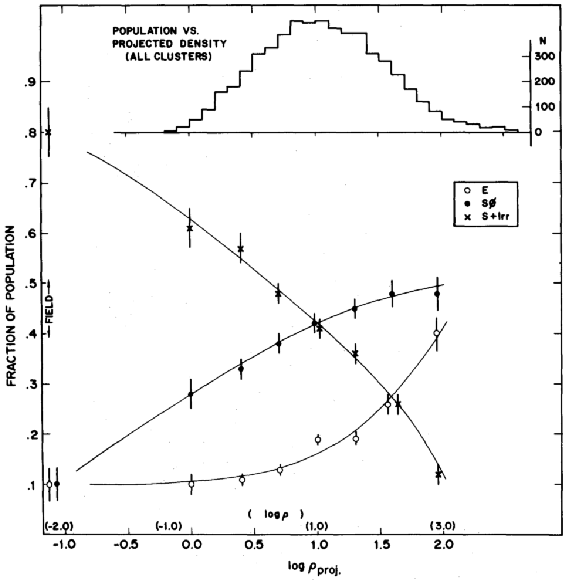
\includegraphics[width=.48\textwidth]{Dressler-morph-dens.png}
   \caption{\small  Simulation showing filaments feeding cluster. data showing how red fraction changes with environment.}
     \label{fig1}
 \end{figure}



%\noindent  \underline{What can Filaments do to a Galaxy?} 
Hydrodynamic simulations of cluster infall regions predict that
the regions in filaments with the highest density gas can enhance the ram pressure in
filaments by up to a factor of $\sim 100$ \citep{bahe13}.  This 
means that freshly infalling galaxies with $\log(M_\star)<9.5$ near a massive
cluster can be stripped of their cold gas even well outside the virial
radius.  For more massive galaxies and at larger distances from the
cluster, the ram pressure in filaments is still sufficient to strip
off the hot gas that will replenish the dense star-forming gas,
although it will likely not affect the densest cold gas.  
Filaments may therefore be the key
sites where galaxies are affected by their environments before they fall into
clusters. 





\vspace*{-.8cm}
\section{Gas and Dust Content of Virgo Filament Galaxies}
\vspace*{-.4cm}
We propose to explore the physical properties of
galaxies in the filaments around the Virgo cluster.   Our approach
differs from and complements previous works, as it moves away from the
simple field/group/cluster trilogy. We follow instead the complex
network of galaxies around a well studied cluster.  Virgo is an ideal
target as it is one of the best studied clusters.  However, there is
only sparse data on galaxies in the well-defined filaments leading
into Virgo from large radii, making our project especially timely.
The study of these filaments will benefit from the comparison with the rich
ensemble of data already obtained for the center of Virgo: the atomic
gas with the VLA by Chung
et al (2009), and also at large scale with ALFALFA \citep{giovanelli05}; the
dust content with the Herschel Virgo Cluster Survey \citep{davies10}; the stellar mass with the
NGVS survey and WISE \citep{ferrarese12}; and recent star formation
from UV data with GALEX GUViCS survey \citep{boselli11}. 




% \noindent \underline{The North-East Filament.} We selected the highest contrast and longest filament existing around
% Virgo. It is relatively straight over 20Mpc and extends up to 7 virial
% radii from the cluster center.  Only a small part of this filament is included in
% the Extended Virgo Cluster Catalog (EVCC), which covers 725 deg$^2$ or 60
% Mpc$^2$.  The EVCC is about 5 times larger than the surface of Virgo
% proper and extend to 3.5 virial radii, but fails to probe the extended filamentary structure around this cluster. 




\begin{figure}[h]
\centering
%\includegraphics[width=0.6\textwidth]{Virgo_positions_boselli.png}
%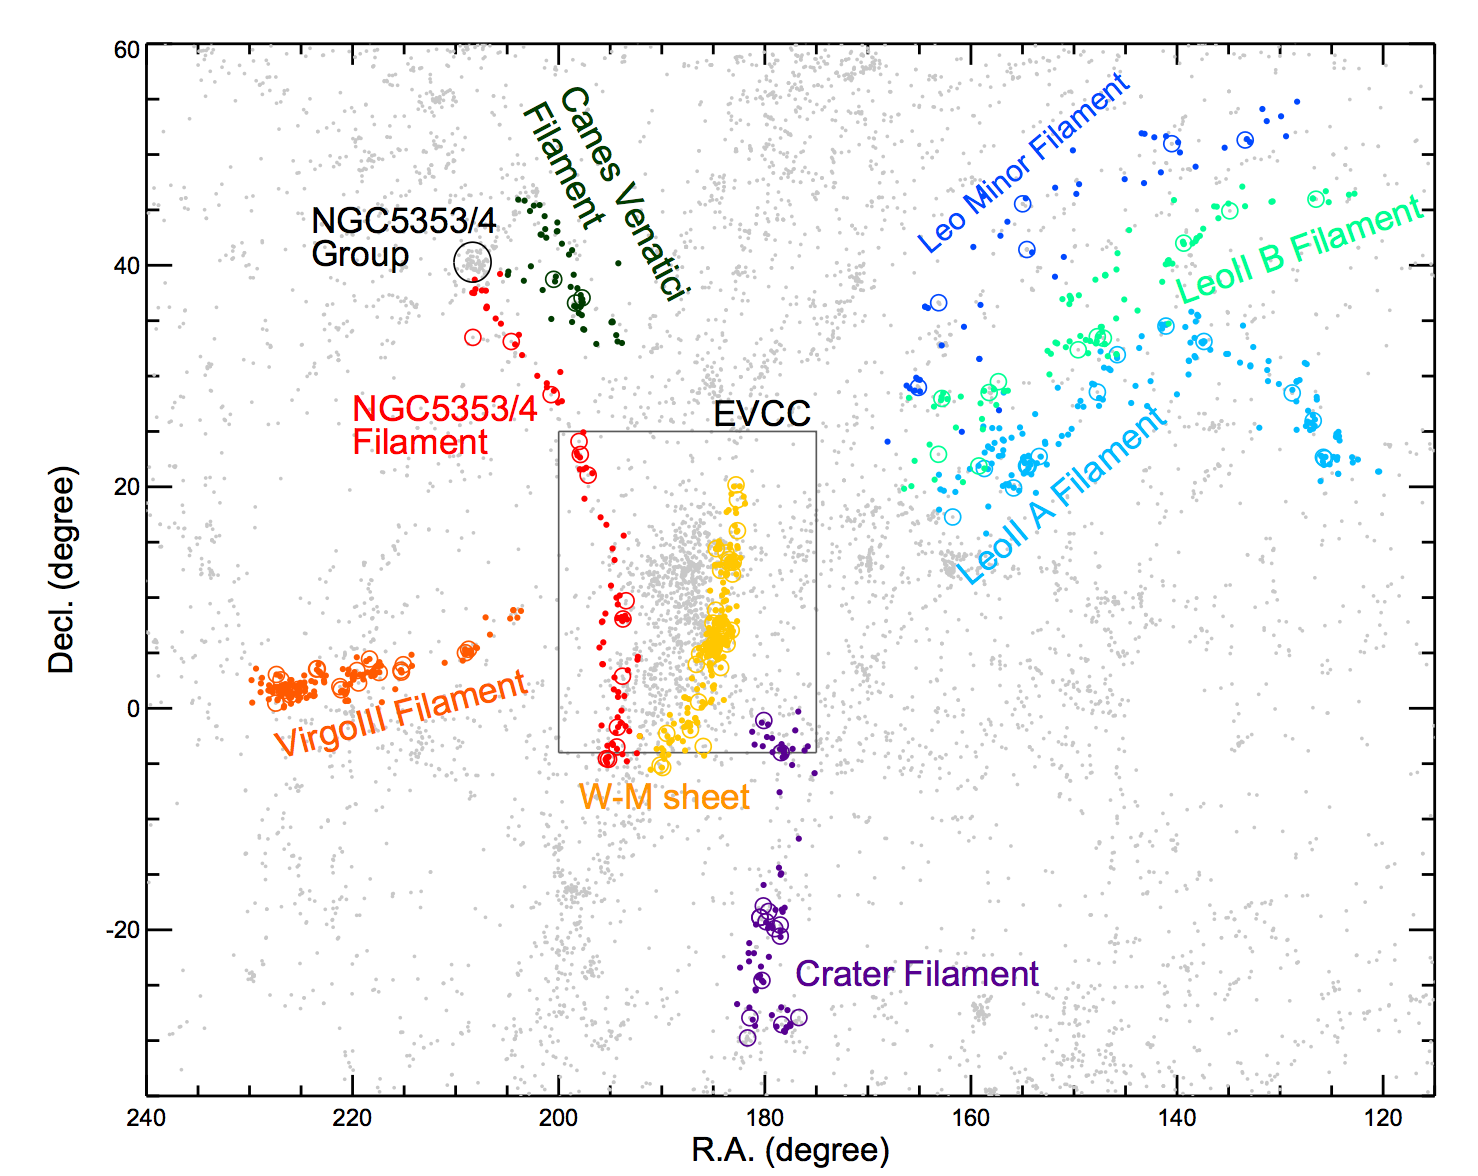
\includegraphics[width=0.48\textwidth]{KimFig1.png}
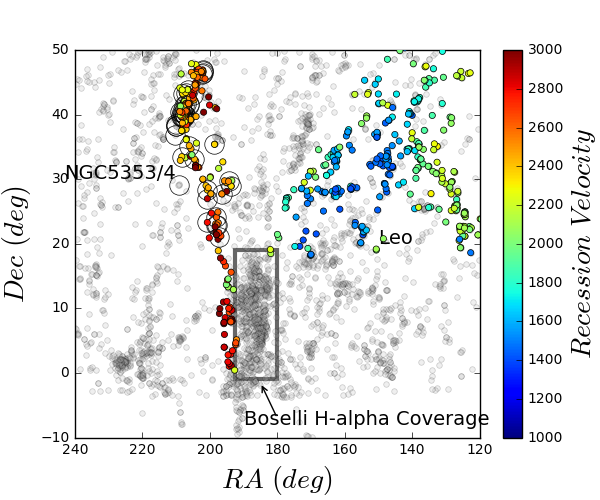
\includegraphics[width=0.48\textwidth]{filaments.png}
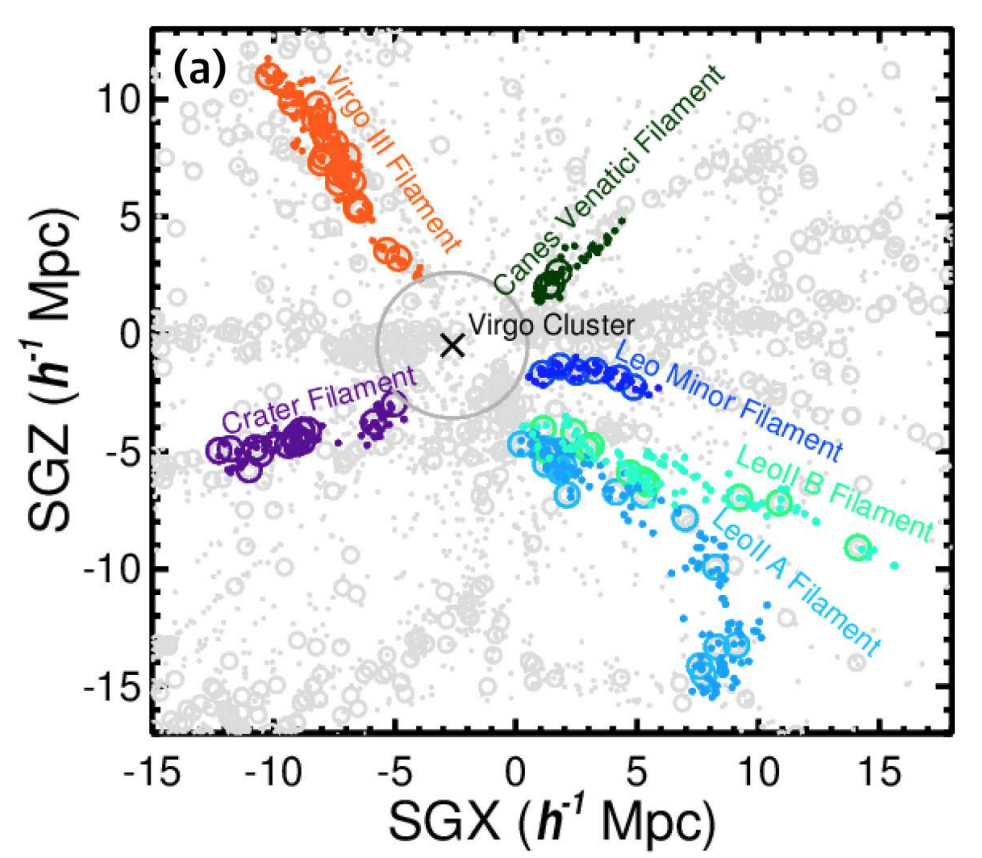
\includegraphics[width=0.4\textwidth]{KimFig2a.png}
\caption{\small {\it (Left)} Figure 1(a) from \citet{kim16} showing filaments
  surrounding Virgo Cluster as observed on the plane of the sky in RA and Dec.  {\it (Right)} Figure
  2(a) from \citet{kim16} showing the same galaxies but projected into
Virgo-centric coordinates.  The Leo filaments can now be seen as three
distinct filaments.  The NGC5353 filament, which does not intersect
the Virgo Cluster, is not shown in the right panel.}
\label{kimfigure}
\end{figure}

% \begin{figure}[h]
% \centering
% 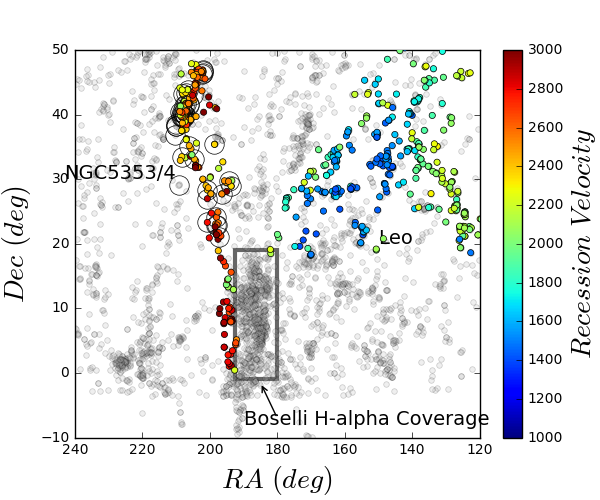
\includegraphics[width=0.6\textwidth]{filaments.png}%{Virgo_positions_NSF.png}
% \caption{%{\it (Left)} 
% Figure from \citet{kim16} showing filaments surrounding Virgo Cluster. {\it (Right)} Galaxies in the vicinity of the Virgo
% Cluster.  The main Virgo cluster is near $RA = 190$
% and $Dec = +10$. The black rectangle shows the NE filament that is the subject of this proposal.
% Galaxies in this filament have recession velocities in the range $2400 < v_r <
% 3000$~ km/s.  The gray rectangle shows the coverage of the
% Boselli large \ha \ imaging program at CFHT that will start in 2017A. It is restricted to the vicinity of the main
% cluster and will not probe galaxies along the filament where
% preprocessing is thought to happen.  The Boselli program will provide
% a useful comparison for our sample of filament galaxies.}
% \end{figure}

% \begin{figure}[h]
% %\includegraphics[width=0.48\textwidth]{Virgo_filament_Halpha_obs.eps}
% \includegraphics[width=0.6\textwidth]{Virgo_filament_CO_obs.png}
% \caption{Zoomed-in view of the filamentary structure to the NE of Virgo.
% The grey points show all galaxies in redshift range $2400 < v_r <
% 3000$~km/s.  The color points show the galaxies we are targeting
% with \ha \ emission.  These 20 galaxies will have CO observations,
% and have $S/N(22 \mu m) > 2$ and $9 < \log_{10}(M/M_\odot) < 10$;
% the points are colored according to stellar mass.
% The black squares (just slightly larger than the colored points) show the 17 HDI pointings that are required
% to image the 20 star-forming galaxies. }
% \label{fig1}
% \end{figure}



% We request time for 22 pointings in 10 groups (2 pointings for most
% groups, 
% 3 for the nearest two groups). With overhead 
% (including 5 exposures per filter to dither over MOSAIC gaps,
% pointing, and focus checks), 
% we estimate 2.5h per field = 55h for 22 fields. In addition we will
% obtain 2-3 spectrophotometric standards and 3 Landolt standard fields
% per night in each filter on photometric nights, requiring ∼0.5 hours
% per night. These observations may be carried out in astronomical twilight.
% We thus request 7 nights, assuming ∼8.5 hours of astronomical twilight per night.
% We do not require dark time for these observations, but bright
% moonlight makes it difficult to detect the outermost parts of the
% galaxies. We therefore request time at least 7 days from full moon.

 
% \ha \ falls perfectly into \ha$+4$nm.

\vspace*{-1cm}\subsection{The Filament Galaxy Sample} 
\vspace*{-.4cm}
\citet{tully82} first studied the large-scale structure around the Virgo
cluster and identified several concentrations of galaxies that he
termed clouds.  More recently \citet{kim16} repeat this analysis with
a much larger spectroscopic dataset that probes to lower luminosities,
and they are able to identify multiple
filaments around Virgo, some that lead directly into the cluster and
others that are nearby but not falling into Virgo.  We show these
filaments in Figure \ref{kimfigure}.
This proposal focuses on two of the filaments identified by
\citet{kim16}, and we highlight these in the bottom panel of Figure
\ref{fig1}.  The NGC5353 filament feeds the NGC5353 group and extends over 20~Mpc,
passing close to but not into the Virgo cluster \citep{kim16}.  The second filament
that we will study is the Leo filament.  \citet{kim16} show that once
you project galaxies into a Virgo-centric coordinate system (see right
panel of Figure \ref{kimfigure}), galaxies
in this region exist in three distinct filaments.  We will target all
of these.  We focus on
the NGC5353 and Leo filaments for two practical reasons:  (1) these filaments
extend the furthest north on the plane of the sky, and this allows
for a longer observing window from northern hemisphere telescopes, (2)
these filaments are among the most distant of the Virgo filaments and
thus the galaxies have smaller apparent size.  This helps to minimize
the aperture correction that we need to apply to CO observations
because when the galaxy size extends beyond the beam size.  






We show the $NUV-r$ color versus stellar mass in Figure \ref{sample}.
The grey circles show all the filament galaxies that are in the
NASA-Sloan Atlas.  The green points show points
that we will target with CO observations.  We have restricted the mass
range for the CO sample to $9 < \log_{10} (M_\star/M_\odot) < 10$.
Galaxies below this mass limit are difficult to detect in CO due
to lower metallicity and photodissociation of CO (ref).  We set the
upper limit to the mass range because we expect that galaxies with
$\log (M_\star/M_\odot) < 10$ will be most affected by the
environment.  We will push above this mass limit as telescope time
permits.

The blue circles in Figure \ref{sample} show galaxies that we will
target with \ha \ imaging.   The \ha \ subsample includes all galaxies
with $8.5 < \log_{10} (M_\star/M_\odot) < 10$.  A total of 95 of these
are in the NGC5353 filament and the remaining 126 are associated with
the Leo filaments.  The observations, data reduction, and analysis of
the \ha \ imaging comprises the main thrust of this proposal.

The second main goal of this project is to map the spatial
distribution of dust within the filament galaxies using WISE 12\micron
\ imaging.   The open red circles in Figure \ref{sample} show 184 galaxies that are
detected at 12$\mu$m by WISE with a signal-to-noise ratio above 10.
We set this as the lower limit so that we have sufficient signal for
fitting a two-dimensional \sers \ model, and we discuss the details of
our image fitting in Section \ref{wise}.


\begin{figure}[h]
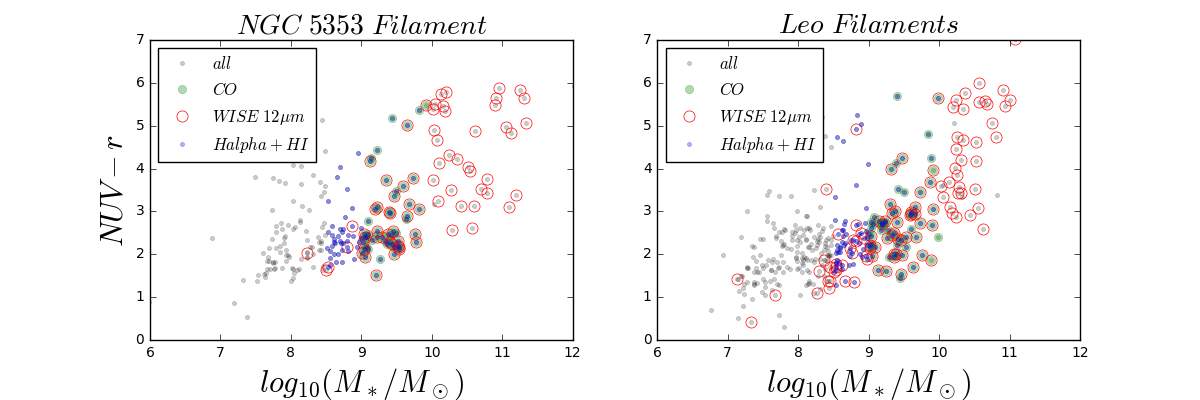
\includegraphics[width=\textwidth]{sample.png}
\caption{\small $NUV-r$ color versus stellar mass for galaxies 
  in the (left) NGC5353 filament and the (right) Leo filaments.
The grey circles show all the filament galaxies that are in the
NASA-Sloan Atlas, and the red circles show all galaxies that are
detected at 12$\mu$m by WISE with a signal-to-noise ratio above 10.
}
\label{sample}
\end{figure}


\vspace*{-.8cm}\subsection{Methodology} 
\vspace*{-.2cm}
Several groups have shown the power of panchromatic galaxy surveys -
SINGS, THINGS, LITTLE THINGS - for understanding the complicated
interplay between warm and cold interstellar medium.  We take a
similar approach, providing a complete census of cold gas and dust,
and look at how the filament environment affects the many components a galaxy's gas reservoir.

and here we propose \ha \ imaging to map the
  spatial distribution of the hot gas and derive integrated SFRs.  The
combination of \ha \ and CO observations will allow us to calculate
gas consumption timescales, characterize multiple phases of the
galactic gas, and look for signatures of environmentally-driven
depletion.
\subsubsection{Molecular and Atomic Gas}
exising CO observations for 80 galaxies in filament

XX of galaxies the three filaments have existing HI detects.

Some observations already planned to observe the remaining galaxies.

HI observations proposed; remaining from green bank

\underline{CO, IR, and Optical Observations:}  {\it We have approved
  CO(2-1) and (1-0) observations with the IRAM 30-meter telescope to
  characterize the molecular gas contents of 20 galaxies the Northeast filament, }
We will quantify the stellar and dust components using
SDSS imaging, optical spectroscopy, and
far infrared (WISE and/or IRAS) fluxes.  Cutting off the hot gas supply or stripping the diffuse molecular gas
is a likely precursor to the suppression of star formation as the
galaxy will use up its cold gas on a timescale of $\sim 2.3$~Gyr
(Bigiel et al. 2011).  Likewise, direct stripping of the cold gas will
result in a suppression of the CO and infrared luminosity and
truncated \ha \ emission (e.g. Koopmann et al. 2004).  Therefore,
we expect a variety of gas effects to be observable by observing a
sample of galaxies in both \ha \ and CO.
Note that Virgo is the closest relatively massive cluster. There is no counterpart
in which the major question of the origin of star formation quenching could be
addressed in such exquisite details.


\begin{figure}[h]
\centering
%\includegraphics[width=0.6\textwidth]{Virgo_positions_boselli.png}
%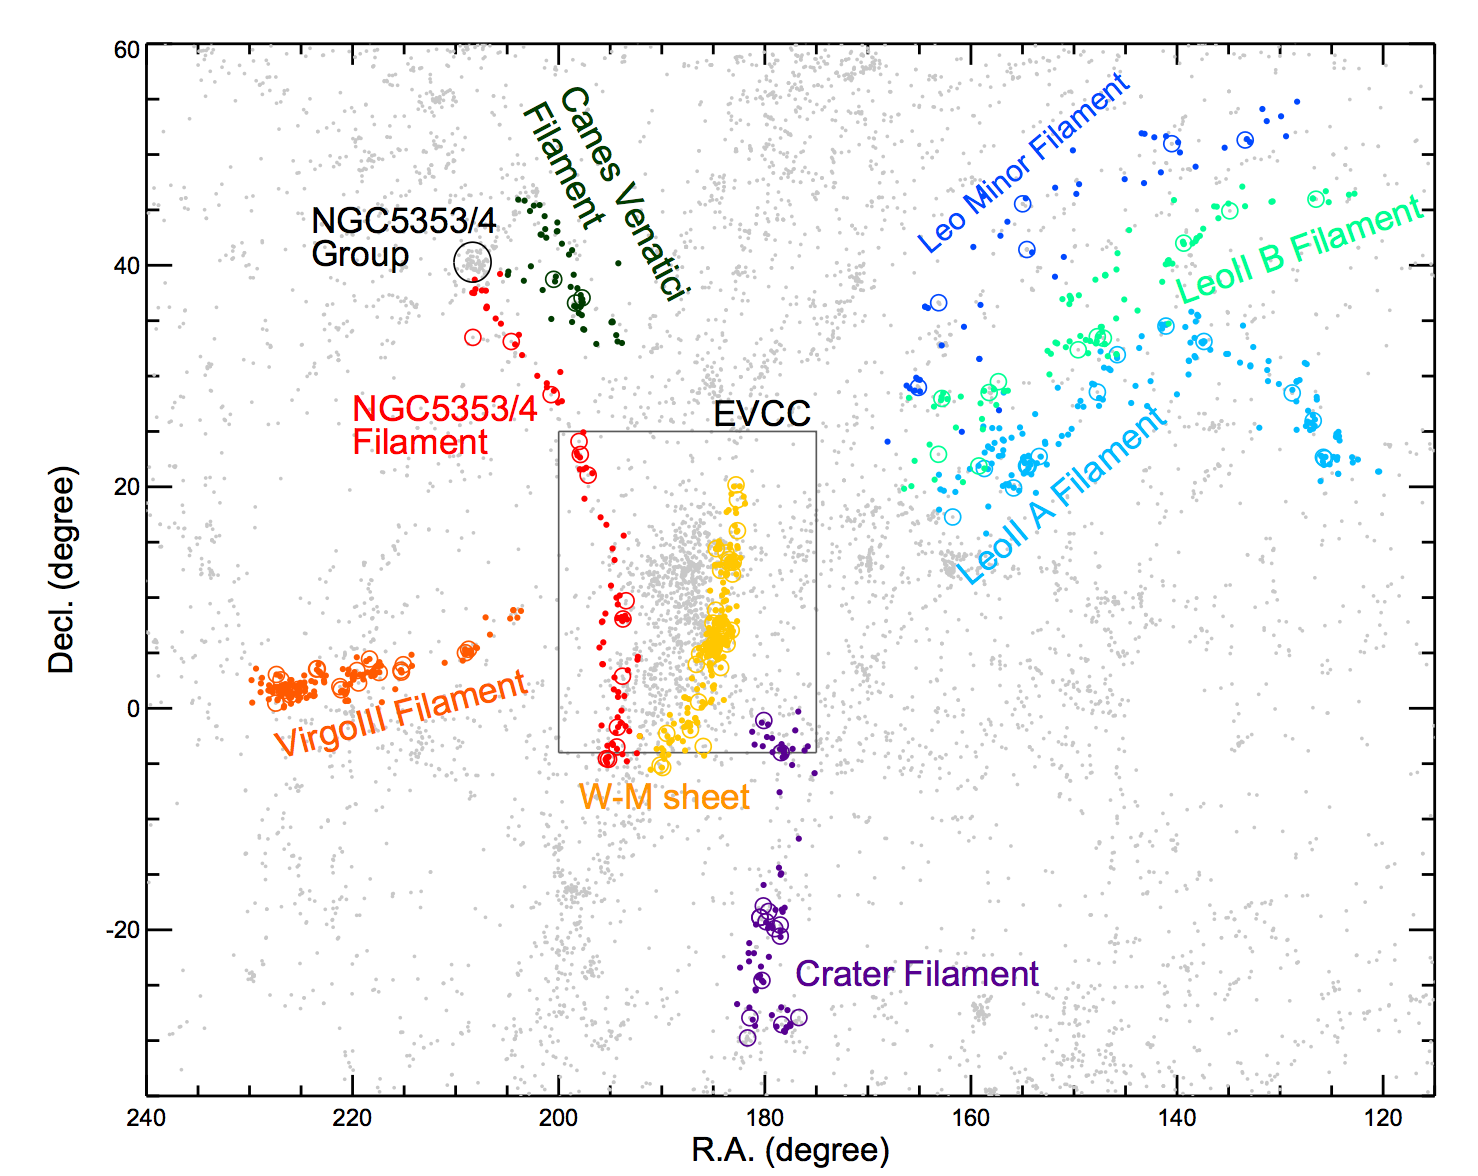
\includegraphics[width=0.48\textwidth]{KimFig1.png}
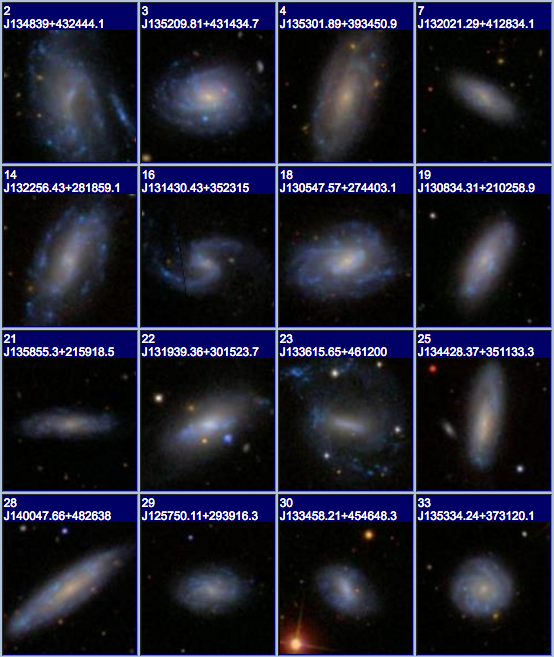
\includegraphics[width=0.48\textwidth]{sdss-montage.png}
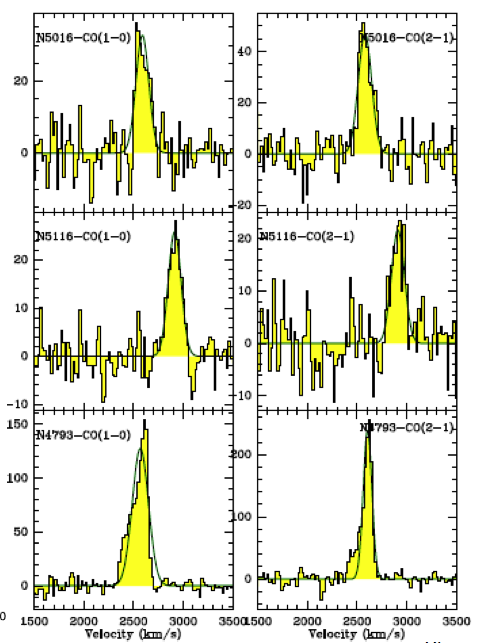
\includegraphics[width=0.4\textwidth]{CO-detection.png}
\caption{\small {\it (Left)} SDSS color images showing 16 randomly
  selected galaxies in NGC5353 filament.  {\it (Right)} CO spectra
  from IRAM 30-m telescope for galaxies in the NGC5353 filament.  }
\label{kimfigure}
\end{figure}


\subsubsection{Ionized Gas and Current Star Formation Rates}



The goal of our program is to obtain spatially resolved \ha \ maps for 222 star-forming galaxies in
the NGC5353 and Leo filaments. These maps will allow us to test specific quenching
mechanisms that involve the removal or rapid consumption of gas from galaxies. Key to accomplishing
these goals are that we are able to measure \ha \ profiles to low surface brightness and that we can
probe galaxies at different positions along the filament out to large
distances from Virgo.
\begin{figure}[h]
\centering
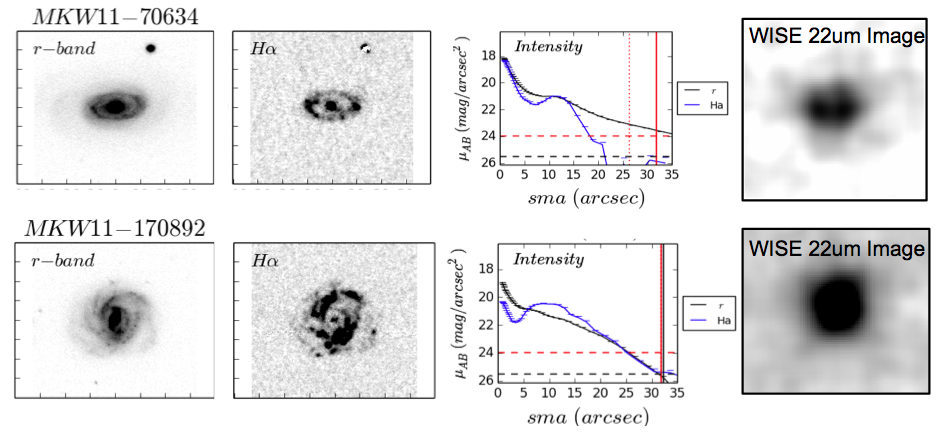
\includegraphics[width=.85\textwidth]{HalphaProfileWISE.png}
\caption{\small
% \textit{Left:} SDSS $gri$ color composites of the 20 galaxies
%   in our $CO-H\alpha$ sample. \textit{Right:}  
To illustrate our proposed \ha  analysis, we show
imaging taken with the KPNO 0.9-m$+$HDI of two galaxies within the
nearby group  MKW11 ($v_r = 6900$~km/s). The left column shows a
galaxy for which the star-forming disk probed by \ha \ is truncated
along the semi-major axis (sma)  relative to the stellar disk as
probed in the $r$-band. The right column  shows an example that is not
truncated.  The SFR is resolved  at about 1/10 of a kpc in \ha. In
contrast, the WISE PSF is 12 arcsec, corresponding to about 1~kpc. The image thumbnails in each row are the same size, demonstrating
that the WISE data are not sufficient to measure the extent and
morphology of the star formation.   Indeed, the WISE photometry may
underestimate the SFR for  the lowest mass galaxies in our sample
because of their low metallicity.  As these galaxies are likely the
most susceptible to stripping, \ha\ imaging is necessary to understand
how environment affects their gas.}
\label{fig3}
\end{figure}


We will complete the \ha \ observations at the WIYN 0.9 and the Mt
Laguna Observatory - Kansas has guaranteed time on the 1.2 m.
For the WIYN 0.9 m, we will apply for time through NOAO, requesting
approximately 6 nights each spring for the three years covered by this
proposal.  Based on past \ha \ imaging experience with the WIYN 0.9 m,
we need about 2 hours per target, and so we expect to be able to
complete 4 objects per night and 24 pointings per run.  Our yield will
be slightly higher ($\sim 30$) because we will be able to place multiple objects within
te $0.5^\circ \times 0.5^\circ$ field of view.  Thus we expect to
complete \ha \ imaging for
$\sim 100$ galaxies at the WIYN 0.9m. 

We will observe the remaining 120 galaxies in the \ha \ sample using the
XX telescope at the Mount Laguna observatory.  
*** Background from Greg - commissioning, camera, FOV**
% 8 hrs per night, 4 objects per night = 24 objects per run
We have included funds to purchase an identical 
$H\alpha+4$~nm filter for this telescope.  


To properly probe any environmentally-driven quenching, we must detect galaxies
with star-formation rates below the star-forming main sequence. Elbaz et al. (2011) find that a
$\rm \log_{10}(M_\star/M_\odot) = 9$ galaxy has a SFR 
of $\rm 0.25~ M_\odot/yr$ at $z = 0$. 
The detection limits of our \ha \ imaging will allow us to detect galaxies with star-formation rates a
factor of ten below the star-forming main sequence.

% Our goal is to probe galaxies with
% SFRs a factor 10 below the main sequence SFRs. 
% We convert our expected surface-brightness sensitivity to a SFR by
% first converting to a luminosity and then using the
% Kennicutt (1983) conversion:
% $\rm SFR(H\alpha)~ (M_\odot/yr)=7.9 \times 10^{-42}~L(H\alpha)~ (ergs/s)$.
% We also assume that the star formation is spread over a circular area
% of 30\arcsec \ radius (see Figure 2).  This corresponds to an integrated
% star-formation rate of $\rm SFR \approx 0.1~M_\odot/yr$.  We will
% therefore be able to detect galaxies with star-formation rates a
% factor of ten below the star-forming main sequence.
% %To select galaxies above this limit, we require a
% %WISE SNR greater than 2 at 22μm. This corresponds to a minimum SFR of
% %$\rm 0.02 M_\odot/yr$ (e.g. Chary \& Elbaz 2001).


{% \bf Fix to reflect larger sample.}
% When possible we put multiple filament targets in the same HDI
% field of view.  We are able to target the complete CO sample of 20 galaxies in 17 pointings. With overhead 
% (including 3 exposures per filter, pointing, and focus checks), 
% we estimate 2.5h per field for a total time of 42.5h. In addition we will
% obtain 2-3 spectrophotometric standards and 3 Landolt standard fields
% per night in each filter on photometric nights, requiring $\sim 0.5$ hours
% per night. These observations may be carried out in astronomical twilight.
% We thus request 6 nights, assuming $\sim 8.5$ hours of observing time per
% night.  
% We do not require dark time for these observations, but bright
% moonlight makes it difficult to detect the outermost parts of the
% galaxies. We therefore request time at least 7 days from full moon.

%\vspace*{-.4cm}\subsubsection{The Local Cluster Survey}

We will measure the radial extent of the \ha \ emission and compare
that to the extent of the stellar disks.
Observations of the nearest galaxy clusters provide 
ample evidence that environment actively alters the gas content of infalling galaxies.  
%satellite vs. central \citep[e.g.][]{omand14}.
Studies of the Virgo cluster show evidence of cold gas stripping
\citep[e.g.][]{koopmann98, koopmann04, dale01, crowl05, chung07,
  corbelli12}, including truncated H$\alpha$ emission of Virgo spirals
compared with their field counterparts \citep{koopmann04}.
We will also measure integrated SFRs and use these to compute gas
consumption times.



\vspace*{-1cm}
\subsubsection{Dust Masses and Spatially-resolved Dust Maps}
\vspace*{-.3cm}
\label{wise}
Infrared images are required to measure the spatial extent of
dust-obscured star formation (and therefore the cold gas). WISE has
observed the entire sky from 3.6-22 micron, providing the data required to make 
size measurements for a statistically significant galaxy sample spanning a
large range of environments. While the WISE PSF is rather large
(6.5\arcsec \ at 12\micron), it
still probes down to $2-5$~kpc for galaxies in the redshift range we are
focusing on, and is sufficient for this study. In constrast, Spitzer
and Herschel data can be much more sensitive. However, they did not
observe these filaments. Nevertheless, Spitzer and Herschel data will be used to validate the
results based on the lower-sensitivity WISE data. In addition to
providing a measure of the spatial extent of star formation, the WISE
colors can be used to indicate the presence of an AGN.  Along with the SDSS fiber
spectroscopy, the WISE colors will be used to eliminate galaxies with
infrared size measurements that are likely to be affected by an AGN.


% This proposal rests on the assumption that 12\micron \ emission, in
% the absence of an active galactic nucleus, traces the star-forming and
% thus gas-rich regions of a galaxy.  This is clearly the case for
% 24\micron \ emission \citep[e.g.][]{calzetti07}, and so here we show
% evidence that the 12\micron \ emission (1) is comparable in extent to the
% 24\micron \ emission, and (2) can differ significantly from the stellar
% disk in terms of extent and morphology. 

we provide a qualitative example.  In Figure
\ref{nsa88353}, we show a spiral galaxy with 12\micron \
emission that is comparable in extent to the stellar disk.  Again,
comparing the $r$ and 24\micron \ images shows a more extended
star-forming disk, and the best-fit \sers \ models indicate that the
24\micron \ emission has an effective radius that is 90\% of the
stellar radius.  Importantly, the 12\micron \ emission is again
comparable in extent to the 24\micron \ emission.


% \begin{figure*}[h]
% \begin{center}
% 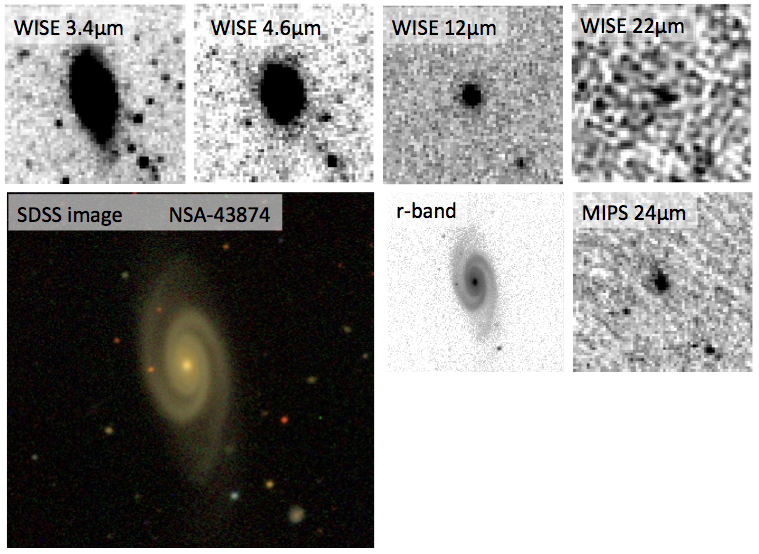
\includegraphics[width=.85\textwidth]{NSA-43874.png}
% \end{center}
% \caption{ Multi-wavelength images of spiral galaxy NSA-43874.  The top
%   4 panels are the WISE images.  The second row shows, from left to
%   right, the SDSS color, SDSS $r$, and MIPS 24\micron \ cutouts.  This
% galaxy has 24\micron \ emission that is truncated relative to the
% stellar disk ($r$-band).  The 12\micron \ emission is comparable in
% extent to the 24\micron \ emission and thus makes a suitable probe of
% the star-forming disk.}
% \label{nsa43874}
% \end{figure*}

\begin{figure*}[h]
\begin{center}
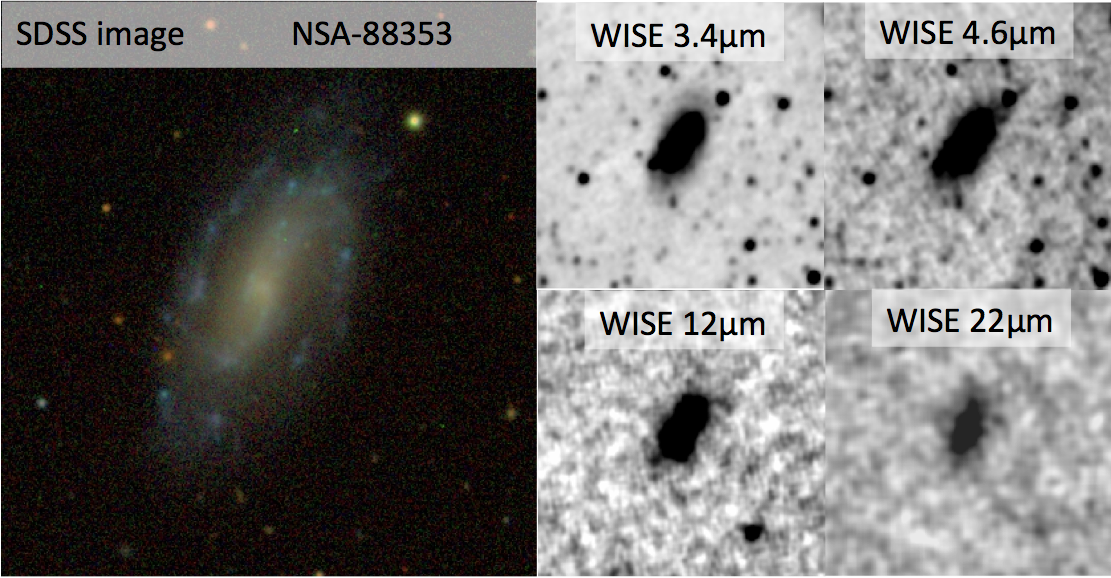
\includegraphics[width=.85\textwidth]{NSA-88353.png}
\end{center}
\caption{ Multi-wavelength images of spiral galaxy NSA-88353.  The 
  4 panels on the right are the WISE images. This
galaxy has 24\micron \ emission that is comparable in extent to the 
stellar disk ($r$-band).  The 12\micron \ emission is comparable in
extent to stellar emission seen in SDSS and 3.4 microns. .}
\label{nsa88353}
\end{figure*}

The above examples show qualitatively that the 12 and 24\micron \ emission
have a similar spatial extent.  To provide a quantitative example, 
we show a preliminary GALFIT analysis for the 12\micron \ image of one spiral
galaxy in Figure \ref{nsa113482}.  The top panel shows the results for
the 12\micron \ image, and the bottom set of images shows the best-fit
for the 24\micron \ image.  The best-fit models, shown in the center
panels, have effective radii that agree within the errors.  Thus, we
conclude that the
12\micron \ images provide a suitable means of tracing the extent of
the star-forming disk.   

\begin{figure*}[h]
\begin{center}
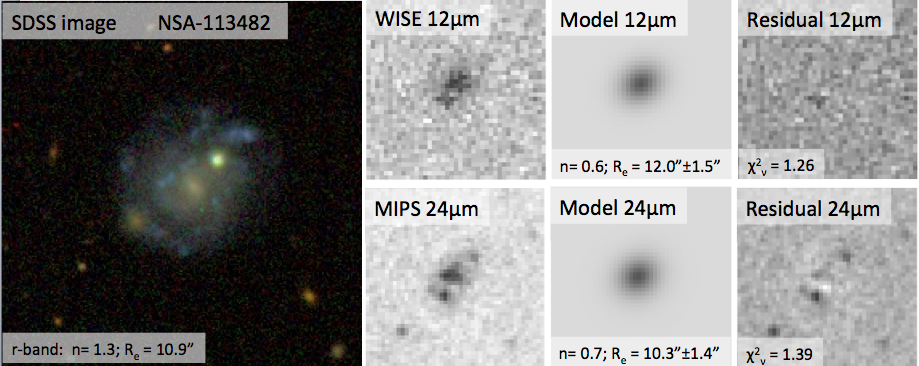
\includegraphics[width=.85\textwidth]{NSA-113482.png}
\end{center}
\caption{ Color SDSS image of spiral galaxy NSA-113482 (left).  The top
  row of three images shows the preliminary GALFIT
  analysis for the 12\micron \ image (top row).  The three images show
the 12\micron \ image (left), the GALFIT model (center), and the
residual after the model is subtracted from the image.  The bottom
panels show the same for the MIPS 24\micron \ image.  The model panels
list the \sers \ profile and effective radius of the best-fit model,
and the effective radii from the 12 and 24\micron \ fits agree within
errors.  This shows that 12\micron \ is a suitable means of tracing
the extent of the star-forming disk.}
\label{nsa113482}
\end{figure*}



The image fitting is already avalaible for the $r$-band images from
the NASA-Sloan Atlas \citep{blanton11}.  Thus the main thrust of this proposal is to run
GALFIT on the 12\micron \ images to measure the spatial extent of the
star-forming disk.  We are not able to use the 22\micron \ data for
this purpose due to
its lower resolution and sensitivity.
To quantify the extent of the 12\micron \ emission, 
we will use  {\it GALFIT} software \citep{peng02}
to fit two-dimensional \sers \ models to the galaxy images.  
We will use {\it unWISE} image products and PSFs \citep{lang14}.
We will use the best-fit parameters from the $r$-band as the initial
guess for the 12\micron \ fits, holding PA and axis ratio fixed at the
optical values.  To test the sensitivity of our results to these
initial conditions, we will stochastically vary  the intial
conditions to provide more robust estimates of range of acceptable
fit parameters.  This process is described in more detail below.

% GALFIT requires a PSF image to properly model galaxies, and this is
% particularly important when modeling low-resolution data such as the
% 12\micron \ images.  We will use a nearby point source for each
% galaxy, choosing a bright, isolated source that shows a
% clear diffraction pattern.

We will use simulated galaxies to test the reliability of our GALFIT
model parameters.  The WISE 12\micron \ data have lower resolution and
lower signal-to-noise ratios than the optical imaging that
GALFIT is typically used with. To test the reliability of the GALFIT models, 
we will create 1000 model galaxies 
and run them through our analysis.
The model galaxies consist of single-component \sers \ models with
randomly-selected parameters.
The model galaxy will be created by first selecting 
a region on a WISE 12\micron \ tile that doesn't have a nearby object within 15
pixels.  We will create a cutout of this region, generate a model galaxy
using GALFIT, and then add 
the model and noise to the WISE cutout.
We will then run the model through our analysis pipeline and compare
the input and recovered parameters.  This will help us determine the
surface brightness limit of our survey.


\vspace*{-1cm}
%\subsubsection
\subsection{Comparison with Theory}
\vspace*{-.4cm}

Constrained Local UniversE Simulations (CLUES) of local
volume\footnote{https://www.clues-project.org} includes dark matter,
gas and stars.




The first scenario we must consider is whether our results are
consistent with predictions of gas depletion through starvation and
the consumption of the remaining gas
rather than more extreme environmental processes such as ram-pressure stripping.
In the left panel of Figure \ref{lizhi_comparison}, we show the predicted size of the
stellar and star-forming components of $z = 0$ galaxies based on the
semi-analytic models of Xie et al. (2016, in prep).  These models
include starvation but do not explicity include environmental
processes such as ram-pressure stripping.  In the right panel of
Figure \ref{lizhi_comparison}, we show the {\it measured} size of the
star-forming and stellar disks versus stellar mass for the {\it Local
  Cluster Survey} galaxies.  While the size of the stellar disks are
consistent with the model predictions, the size of the star-forming
regions fall systematically below the model predictions.  This
indicates that additional environmental processes must be included to
explain the small observed size of the star-forming region in these
galaxies.  However, the {\it Local Cluster Survey} sample is small and
contains very few isolated/field galaxies.
We need (1) a larger sample of cluster galaxies to confirm the inconsistency between model
and obervations, (2) a larger field sample to serve as a controlled
comparison with the models, and (3) a more robust determination of
the size of the star-forming region that includes a formal analysis of
uncertainty.
\begin{figure*}[h!]
\begin{center}
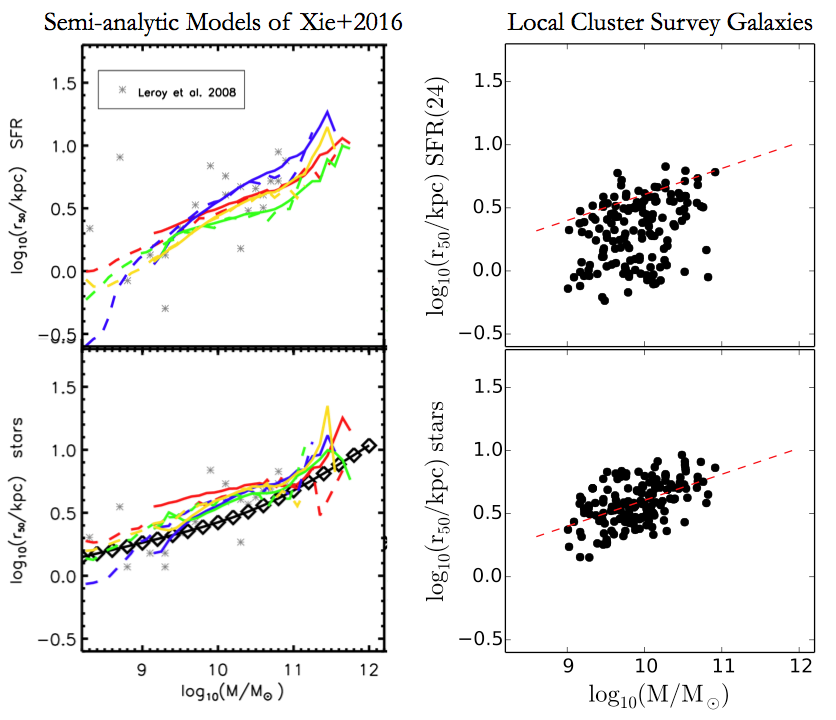
\includegraphics[width=.85\textwidth]{lizhi_comparison.png}
\end{center}
\caption{ (left) {\bf Predicted} half-light radius
  of stars (bottom) and star formation (top) versus stellar mass for
  $z = 0 $ galaxies (Xie et al. 2016, in prep).
  The different color lines represent different models for partitioning
  atomic and molecular hydrogen, and the grey points show comparison
  with some existing observations.  
(right) {\bf Measured} half-light radius of stars (bottom) and star
formation (top) versus stellar mass for galaxies in the {\it Local Cluster Sample}.  The
red dashed line is a linear fit to the stellar half-light radius and
is shown in the top panel for comparison.  The size of the star
forming region is smaller than predicted by semi-analytic models,
suggesting that starvation is not sufficient to explain the observed
size of the SF region in these galaxies.  A larger sample of galaxies
with more robust size measurements is needed to confirm this result.}
\label{lizhi_comparison}
\end{figure*}



Theoretical models of ram-pressure stripping provide predictions that
we can compare directly to our measurements.
For example, numerical simulations of starvation and ram-pressure stripping of cold gas 
generically predict that star formation in the edges
of galaxies will be affected more strongly than star formation near the
centers of galaxies; the spatial extent of the star-forming disk
should be smaller for galaxies that are undergoing stripping \citep[e.g.][]{kawata08, bekki14}.
We find evidence of this in the {\it Local Cluster Survey}, but we
also find a stronger correlation with bulge-to-total ratio.  A larger
sample is needed to disentangle these effects.
In addition, low mass galaxies should be more
vulnerable to having their gas removed 
because the gas in lower mass galaxies is not as tightly
bound \citep[e.g.][]{kawata08, mccarthy07, bekki14}.  We find
some evidence of this in the {\it Local Cluster Survey}, but a larger
sample is needed to strengthen the statistical significance. 

%\vspace*{-1cm}
\subsubsection{Computational Requirements and
  Facilities:   \label{comp}}
\vspace*{-.4cm}
Siena College has recently acquired a High Performance  Computer
Cluster. The cluster %, which is geared primarily towards research
%activities, represents a joint venture by Chemistry, % (Prof. G. Barnes),
%Physics, % (Prof. G. Vernizzi, Prof J. Moustakas) 
%and Computer Science.  %(Prof. Small Research Groups).  
%It 
consists of 16 nodes each with two
Intel Xeon E5-2630 6-core processors and 32 GB of RAM.  The cluster
has a total global storage capacity of 20.5 TB and 208 cores each
running at 2.3 GHz.  
%Several scientific computing software packages
%are installed on the cluster, such as Gamess, NWChem, Gromacs, LAMMPS,
%Octave, Scilab, FFTW, and MySQL Cluster.  In addition T
The Intel
compiler suite is available to create efficient custom programs.


We estimate the computational complexity for analyzing 7000
galaxies with GALFIT in a systematic fashion. We would scan over the
five-dimensional parameter space  p$=$(x,y, radius, concentration,
brightness), by discretizing each dimension from a minimum search
value to a maximum one, and sweeping over the entire mesh of points.
Assuming an average of 10 points per search direction, we have a
lattice with $10^5$ points. Preliminary analyses showed that the average
fitting time is about 20 seconds with GALFIT. Therefore, the total
computational time  for scanning the entire parameter space is of the
order $1.4 \times 10^{10}$ seconds, which is  prohibitively high for the
computational resources at Siena College. However,there is no need to
sample over ALL the points, since we are interested only in the number
of the basins of attraction of each value $p*$. In other words, GALFIT
provides a direct way to map all possible starting points $\{p\}$ to a
subset of points $\{p*\}$ of 'best fit' points. Since the minimization
algorithm used by GALFIT is  the Levenberg-Marquardt algorithm, or
downhill gradient, one can safely assume that around the minimum $p*$,
the best fit function is quadratic. We can therefore estimate the
Hessian numerically around such point and extrapolate the size of the
basin of attraction. In this way we can remove a number of points $\{p\}$
from subsequent sweeps, as they would likely converge to the same attractor
$p*$. We cannot estimate the size of the basins of
attraction precisely, nor the number of minima $p*$, at this stage. For
instance, if we find that only one or two minima exist, then quickly
50\% to up almost 100\% of the points can be skipped in the subsequent
sweeps, because they would not bring any  additional information. The
calculation would be quite fast in this case.  A higher number of
local minima will only be detected by systematically sampling phase space.

We are also considering a stochastic sampling of the parameter space,
by alternating a Monte Carlo sampling with the gradient minimization
algorithm \citep{pardo11}. The code would be serial, but optimized for speed. In this
case, the statistical errors decrease with 1/sqrt(N) where N is the
number of sampling points in the parameter space. If N=1000 the
relative error is of the order of 3\%, which is acceptable. Such an error
is independent from the number of dimensions of the parameter space.
Therefore  stochastic sampling will have a definitive advantage.
By running it on the HPCC of Siena College, it would take about 8
days of computational time. The test and exploratory runs are
anticipated to take an additional 50 CPU hours \citep[for a recent
application of this method see,][]{sala12}.

The two computational techniques described above are sufficient to
create a map of the full phase diagram accurately.  In addition, we
will compare the GALFIT results to those generated by other
independent fitting programs such as 
GALPHAT \citep{yoon11} and The Tractor \citep{lang16}.

\vspace*{-.9cm}\subsection{Workplan, Major Milestones, and Timeline for Completion }
\vspace*{-.3cm}
Rose Finn, Ph.D., is a professor in the Department of Physics
and Astronomy at Siena College (Loudonville, NY).  She is the PI of
the \lcs \ and has extensive experience with running GALFIT on MIPS
24\micron \ imaging.  She will lead the analysis of the WISE 12\micron
\ imaging, lead the \ha \ imaging survey at KPNO, supervise the undergraduate students, and draft the paper.

Vandana Desai, Ph.D., is an astronomer at the NASA/IPAC Infrared
  Science Archive (IRSA).   Vandana has extensive experience
in all aspects of infrared astronomy and will lead technical aspects
associated with the WISE data.  
She also is well-versed in best-practices of data sharing and will
lead our efforts to disseminate data products over the web.

Graziano Vernizzi, Ph.D., is an associate professor at the Department of
Physics and Astronomy of Siena College (Loudonville, NY).
%He has held research positions at the Department of Materials Science
%and Engineering of Northwestern
%University (Evanston, IL), at the Institute of Theoretical Physics
%IPhT) of CEA/Saclay (France), and at the Physics Department of
%University of Oxford (Oxford,UK). In 2007, he received the Cozzarelli
%Prize from the editors of the Proceedings of the National Academy of
%Sciences (PNAS) for the best article in Engineering and Applied
%Sciences. 
His research interests lie in computational and theoretical
physics, biophysics, nanoscale science, soft condensed matter, and
random matrix theory. 
%Recently, he published a chapter in the The
%Oxford Handbook of Random Matrix Theory (Oxford University Press,
%2011) on the application of random matrix theory to the study of
%ribonucleic acid folding.  
Graziano will the lead the computational
aspects of this project.

Gregory Rudnick, Ph.D., is an associate professor at the University of
Kansas.  He has expertise in galaxy evolution, and he is leading an
$HST$ study to measure the spatial extent of star-formation in
intermediate-redshift galaxies.  He will lead the \ha \ imaging survey
at XX observatory.   Will supervise XX students.


Gabriella De Lucia, Ph.D, is a permanent research scientist at INAF -
Astronomical Observatory of Trieste.  Grabriella provides expertise in
semi-analytic modeling of galaxy evolution. She is working on models
that predict the spatial extent of the stellar and star-forming disks,
and her work is thus extremely pertinent to this proposal.  She will lead
the theoretical interpretation of our results and the comparison
with semi-analytic models of gas consumption.

Pascale Jablonka


Francoise Combes, PhD, is a Professor at College de France, and astrophysicist at Paris Observatory. She is an expert in the dynamics of galaxies, their star formation (SF) efficiency and feedback processes, including the action of a super-massive black hole. She has made numerical simulations to test the processes of SF quenching, ram pressure stripping, tidal interaction, or strangulation. She will observe the cold gas content of galaxies in the Virgo filaments, the atomic (HI) or molecular (CO) reservoirs.

A total of 12 Siena College undergraduates students will be involved
in this project over the course of three summers.  During the first
summer, the students will work on cross-matching our galaxy sample
with ALFALFA, GIM2D structural fits, and the unWISE photometric catalogs.  During the second summer, the
students will analyze the star-forming main sequence using the
WISE-derived star-formation rates.

The major milestones and timeline for completion
are listed in Table \ref{schedule}. 
\begin{table}[h!]
\small
\caption{Major Milestones and Schedule \label{schedule}}
\begin{tabular}{|p{.5in}|p{.5in}|p{1.4in}|p{1.in}|p{1.in}|p{1.2in}|}
\hline
\multicolumn{2}{|c|}{\bf Timeline} & \multicolumn{3}{|c|}{\bf Responsibilities} & {\bf Dissemination} \\
\hline
 \multicolumn{2}{|c|}{~~} & Finn & Desai & Vernizzi & \\
\hline
%& & & & & \\
{\bf Year 1 (2017)}& Spring & Finalize sample selection; identify and remove AGN; write code to retrieve cutouts from {\it unWISE}; calculate stellar masses & 
Identify best techniques for modeling WISE PSF & 
Adapt GALFIT code to run on Siena computer cluster; develop code to run image analysis on parallel computing system & \\
\hline
 & Summer & Supervise summer students - cross match sample with other surveys (ALFALFA, GIM2D, unWISE photometry); identify groups and clusters within survey region; calculate environment parameters such as local density & 
Fit IR templates to estimate IR luminosity and SFRs for galaxies & 
Run code on computer cluster for a subset of the sample; adjust code and methodology as needed & \\
\hline
& Fall & Cross-check results with size measurements from MIPS data; run simulations to understand reliability limits &
Interface with NED to plan for web release & 
Run code on complete sample & \\
\hline
{\bf Year 2 (2018)} & Spring & \multicolumn{3}{|c|}{Continue with analysis of full sample.} & 
Poster at Jan 2018 AAS on preliminary results \\
\hline
& Summer & Finalize analysis; supervise summer students (star-forming main sequence as a function of environment);
draft paper &
Help draft paper; supervise web dissemination & 
Help supervise summer students; help draft paper & 
Make data products publically available through NED \\
\hline
& Fall &  \multicolumn{3}{|c|}{Continue with analysis of full sample.} & 
present results at topical meeting;
publish paper; release data to web \\
\hline
\end{tabular}
\end{table}

% \begin{table}[h]
% \caption{Major Milestones and Timeline \label{schedule}}
% %\includegraphics[width=.9\textwidth]{timeline.png}
% %printed from google doc
% \includegraphics[width=\textwidth]{NASA2016-Timeline.pdf}
% \end{table}

\vspace*{-.8cm}\subsection{Data Sharing and Further Dissemination of Results }
\vspace*{-.3cm}
%{\it To facilitate data sharing where appropriate, as part of their technical proposal, the Proposer shall provide a data-sharing plan and shall provide evidence (if any) of any past data- sharing practices.}
We will produce a variety of measurements of the gas content of
filament galaxies.  We will produce a catalog of CO, HI, dust, Halpha
properties to be released with our final paper.

While this data set of derived information will not be exceptionally
large in volume, it will be of value to other observational
astronomers and theorists working on galaxy evolution. To facilitate
the widespread use of these data, we will publish the full catalog of
measured and derived quantities on the web and in the on-line version
of Astrophysical Journal Supplement. In addition, we will work with
the NASA/IPAC Extragalactic Database (NED) to ensure that our data are
discoverable to a larger user base. Co-I Vandana Desai, resident at
IPAC, will act as our NED liason to ensure that this gets done in a
timely manner.

\vspace*{-.7cm}
\section{Broader Impact}

\vspace*{-.4cm}
\subsection{Modeling Physics for High School Programs}
\vspace*{-.4cm}
The modeling
approach is an innovatve and effective way to teach physics that is 
fundamentally different from traditional techniques.  Students are led through
carefully constructed experiments and exercises to clearly develop the conceptual, 
visual, and mathematical models of how physics works.  
Experienced physicists already have these mental models, 
but beginning physics students do not.
These models are essential for understanding physics.
The modeling approach minimizes lectures, and instead 
students are actively engaged in collecting and analyzing real-time data
that illustrate the fundamental concepts of physics.   The students must
then construct models to interpret these
data.  

As a former high school teacher, I know first-hand the importance of 
bringing the more effective and engaging techniques to the front line.
As part of a previous NSF grant (AST-08XX), we have offered 
modeling workshop for high school physics teachers for the past 9 summers.
We are fortunate
to have as an adjunct instructor an area high-school physics teacher who
is an expert in using the modeling approach to teach physics, and
he will continue to lead these workshops.  
We offer 6 hours of continuing education credit to participants 
that can be used toward teacher recertification.
This grant will provide a stipend for Darren Broder to organize and lead
the workshops.  In successive years, Darren's compensation
will be supported by registration fees from participating teachers.
To assess the impact of the modeling curriculum, participating teachers
will administer the force concept inventory and mechanics baseline test.
In collaboration with Darren Broder, I will develop another assessment 
test for Electricity and Magnetism.  

Each spring, the School of Science will help sponsor a dinner for area math and
science teachers.  The goal of this is two-fold.  First, we will have a Siena student
present on a recent research project so that the teachers become better acquainted with
the opportunities for Siena students.  Second, the teachers will have time for informal
conversations to exchange teaching ideas and materials.

\vspace*{-.7cm}
\subsection{Undergraduate Summer Research}
\vspace*{-.4cm}
The importance of undergraduate research is widely recognized
in the science community.
{\em Recent studies have shown that undergraduate research may be the
pedagogy for the 21$^{st}$ century (e.g., Council on Undergraduate Research
Statement and references therein).}
Involvement in research projects
fosters highly motivated, self-confident students with enhanced
analytical and communication skills. 


%The other member institutions are Colgate University,
%Cornell University,
%George Mason University,
%Georgia Southern University, 
%Humboldt State University, 
%Lafayette College, 
%St. Lawrence University, 
%Skidmore College, 
%Union College, 
%University of Puerto Rico, 
%University of Wisconsin, 
%Wesleyan University, 
%and West Texas A\&M University.
% As a team member, myself and participating Siena students
% have attended (Jan. 2008) and will continue to attend the Annual 
% Undergraduate ALFALFA Team Workshop at 
% Arecibo Observatory.  The workshop provides the framework for the program,
% communicating ALFALFA science, observing, and data analysis techniques to
% undergraduate researchers. During the workshop, lectures, observing sessions, and group work 
% are led by %National Astronomy and Ionosphere Center (NAIC)
% %staff, 
% team faculty and graduate students.  
% Siena members will also observe at Arecibo at other times during the year, giving students hands-on experience 
% in using a world-class national facility. 
% In addition, an NSF grant to support the undergraduate consortium has 
% provided money for Siena to purchase a dedicated computer for processing 
% ALFALFA data.  The same NSF grant will provide summer salary for one Siena 
% student every other year.
% However, more students are interested in participating, and therefore, we need more support.


Four Siena students began the first stages of their research projects this summer,
and I expect all of these students to continue their involvement through the next academic year.
Graduating students will be replaced by interested freshman or sophomores to maintain a total
of 4 undergraduate researchers at any one time.  
Specific goals for current and future student researchers are:
\vspace*{-.2cm}
\begin{itemize}
\vspace*{-.25cm}\item learn how to use python for image reduction and
analysis 
%\vspace*{-.25cm}\item learn how to reduce the radio data taken with the Arecibo Radio telescope
%\vspace*{-.25cm}\item identify sources of Hydrogen emission and characterize the properties of the Hydrogen emission, such as the total mass of Hydrogen gas
%\vspace*{-.25cm}\item cross-correlated the Hydrogen sources with existing surveys such as the Sloan Digital Sky Survey and the 2 Micron All Sky Survey
\vspace*{-.25cm}\item identify correlations between optical and Hydrogen properties of galaxies and look for variations in these correlations as a function of galaxy environment
\end{itemize}
\vspace*{-.2cm}


An important part of the research experience is presenting results
to the community.
I will encourage all students 
to present their results at the fall meeting of the 
Astronomical Society of New York and Siena's Academic Celebration, which
is held each spring.  In addition, I will strongly encourage seniors to
present a poster at the 
annual winter meeting of the American Astronomical Society.  

To assess the impact of this project, I will track participation, papers, 
presentation, and post-graduate activity of all Siena students
who are involved in this project.  I will design and implement a survey to 
assess student plans/goals before, during, and after
participation in research.

\vspace*{-.7cm}
\section{Summary}
\vspace*{-.25cm}

{\bf Intellectual Merit:} 
%How important is the proposed activity to advancing knowledge and understanding within its own field or across different fields? 
%How well qualified is the proposer (individual or team) to conduct the project? (If appropriate, the reviewer will comment on the quality of the prior work.) 
%To what extent does the proposed activity suggest and explore creative, original, or potentially transformative concepts? How well conceived and organized is the proposed activity? 
%Is there sufficient access to resources?


{\bf Broader Impact:} This proposal resonates with the National Science Foundation's {broader impacts}
criteria on many levels.  
%How well does the activity advance discovery and understanding while promoting teaching, training, and learning? 
%How well does the proposed activity broaden the participation of underrepresented groups (e.g., gender, ethnicity, disability, geographic, etc.)? 
%To what extent will it enhance the infrastructure for research and education, such as facilities, instrumentation, networks, and partnerships? 
%Will the results be disseminated broadly to enhance scientific and technological understanding? 
%What may be the benefits of the proposed activity to society?
First, the proposal helps promotes teaching and learning by
promoting
modeling approach to teaching HS physics, integrating problem-based learning into general physics,
and the introduction an astronomy 
concentrations within the physics major to increase the number of majors.
Nationally, astronomy traditionally draws a higher fraction of women than physics, so 
the introduction of the astronomy concentration should attract more female students, 
a group that is significantly under-represented in phyiscs.
Second, the project provides hands-on training and learning for tens of 
undergraduate students through research.  
The Siena undergraduate students will be 
encouraged to become involved in all aspects
of research, including data aquisition at world-class observatories, on-campus 
data reduction and analysis, and presentation of results at national
conferences and through publication in peer-reviewed journals.
%The majority of undergraduate physics majors at the
%Siena pursue science jobs in industry after graduation. 
The computer analysis, data interpretation, and presentation skills the
undergraduates learn 
will be essential for success in
the workplace, the classroom, or graduate education in any field of science. 
Finally,
the proposal enhances the infrastructure for research and education at Siena College 
by formalizing collaborations
with the ALFALFA team, several of whom are located in New York State and already serve as an
extended network of mentors for Siena undergraduates.
The proposal will also enable Siena to conduct remote observing sessions at Arecibo.

{\bf Broad Dissemination of Results:} The scientific results of will be disseminated broadly through publication in peer-reviewed journals,
online database, presentation at regional, national and international meetings.  
I will provide a full catalog for the scientific community that will include
an extensive array of primary and derived data products.
%optical and 24\micron \ disk scale length, asymmetry measure, HI mass,
%HI deficiency, properties of ICM as characterized by X-ray luminosity and
%temperature.  
This will be a much-needed reference for galaxy evolution modelers,
particularly those who model the evolution of galaxies. 
The pedagogic results will also be disseminated broadly through 
publication in peer-reviewed journals and presentations at regional and national conferences.  
Of particular interest is the impact that problem-based learning has
on student retention and research readiness.  
In addition, we will develop a new assessment tool that measures a student's
ability to think independently and solve real-world problems.  This
will be of wide interest to institutions looking to implement
similar research-focused curricular changes.

%The undergraduates will complete surveys at 
%the beginning, during, and at the end of their involvement to track
%career goals and the influence that hands-on research experience
%has on those goals.




%The science education major will help adapt existing astronomy 
%labs\footnote{e.g., http://www.astrosociety.org/education.html} 
%to specifically address concepts in the New York State 
%Physics, Earth Science, and Chemistry curricula.
%The labs will be tested at local high schools, presented at 
%Science Teachers Association of New York State meeting, and made
%available on the web.


\clearpage
\bibliography{/Users/rfinn/research/Papers/rfinn}
%\bibliography{/Users/rfinn/bin/bibtex/rfinn}
%\bibliographystyle{nsf}
\bibliographystyle{apj}
%\bibliography

% NOTES:

% look at star formation in dwarfs

% halpha luminosity function

% post-bac student to reduce Halpha

% write reduction pipeline

% summer salary

% filter for Mt Laguna - 

% travel funding for conferences
% group meetings 


% models from Gabriella

% letters of support from Gabriella, Pascale, Francoise


% Halpha + CO - grant 
% size of SF region in different 

% THEORY:
% - spatial distribution of Virgo-like cluster
% - illustrus hydrodynamical simulations
% - compare with CLUES - simulations of local volume


% select sample - determine the amount of observing time required.



% filaments - 

% literature with existing CO observations

% Young+1995
% Brain, Combes + 93
% Sage 93
% Casoli+98
% HERACLES, IRAM CO(2-1)
% ATLAS 3D - Young+2011
% BIMA-song

% filament 3 - 


% Cosmic flows:
% Tully; Courtois

% CLUES - simulations; gas stripping, size of SF region, gas mass (below
% 1E4 K)

% post-processing - compute amount of mass that has been stripped;

% fund:
% observing;
% filter;


\end{document}
